\label{chap:propose}
Phần này sẽ giới thiệu giải thuật đề xuất để áp dụng tiến hóa đa nhiệm giải quyết nhiều mô hình học tăng cường khác nhau.
\subsection{Mã hóa và giải mã cá thể}
Để mã hóa mô hình mạng neural vào một kiểu gen đồ án sử dụng phương pháp sử dụng một nhiễm sắc thể đơn để biểu diễn một policy với các gen là trọng số của mạng Neural như trong hình \ref{fig:problem:policy}. Phương pháp mã hóa và giải mã mạng neural này sẽ dùng phương pháp mã hóa và giải mã đã được trình bày ở chương 3.
\begin{figure}[ht]
    \centering
    \fbox{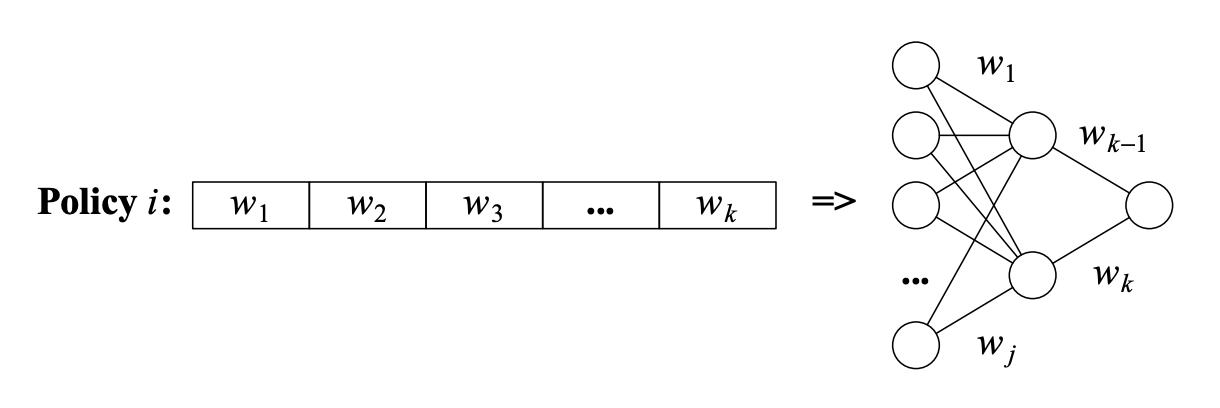
\includegraphics[width=0.7\linewidth]{policy.png}}
    \caption{Cách biểu diễn policy đơn giản bao gồm các trọng số của mạng neural.}
    \label{fig:problem:policy}
\end{figure}
% Một mô hình mạng policy được biểu diễn bởi một cấu trúc mạng $H=(h_1,h_2,...h_k)$ có số lớp là $L$ ta sẽ thực hiện tính toán kích thước của không gian chung tương ứng với cấu trúc mạng này:
% % \begin{align}
% %     D_{chung} = \sum_{l={1,...L}}(h_{l-1}\cdot h_l + h_l)
% % \end{align}

% Các tham số của mạng sẽ được mã hóa lần lượt vào không gian chung này. Khi cần đánh giá fitness trên một biểu cá thể ta sẽ giải mã từ nhiễm sắc thể về các bộ tham số $w$ và độ lệch $b$ tương ứng để tính tổng phần thưởng thu được với bộ tham số này.

\subsection{Xây dựng không gian tìm kiếm chung}
\begin{figure}[ht]
    \centering
    \scalebox{0.85}{\fbox{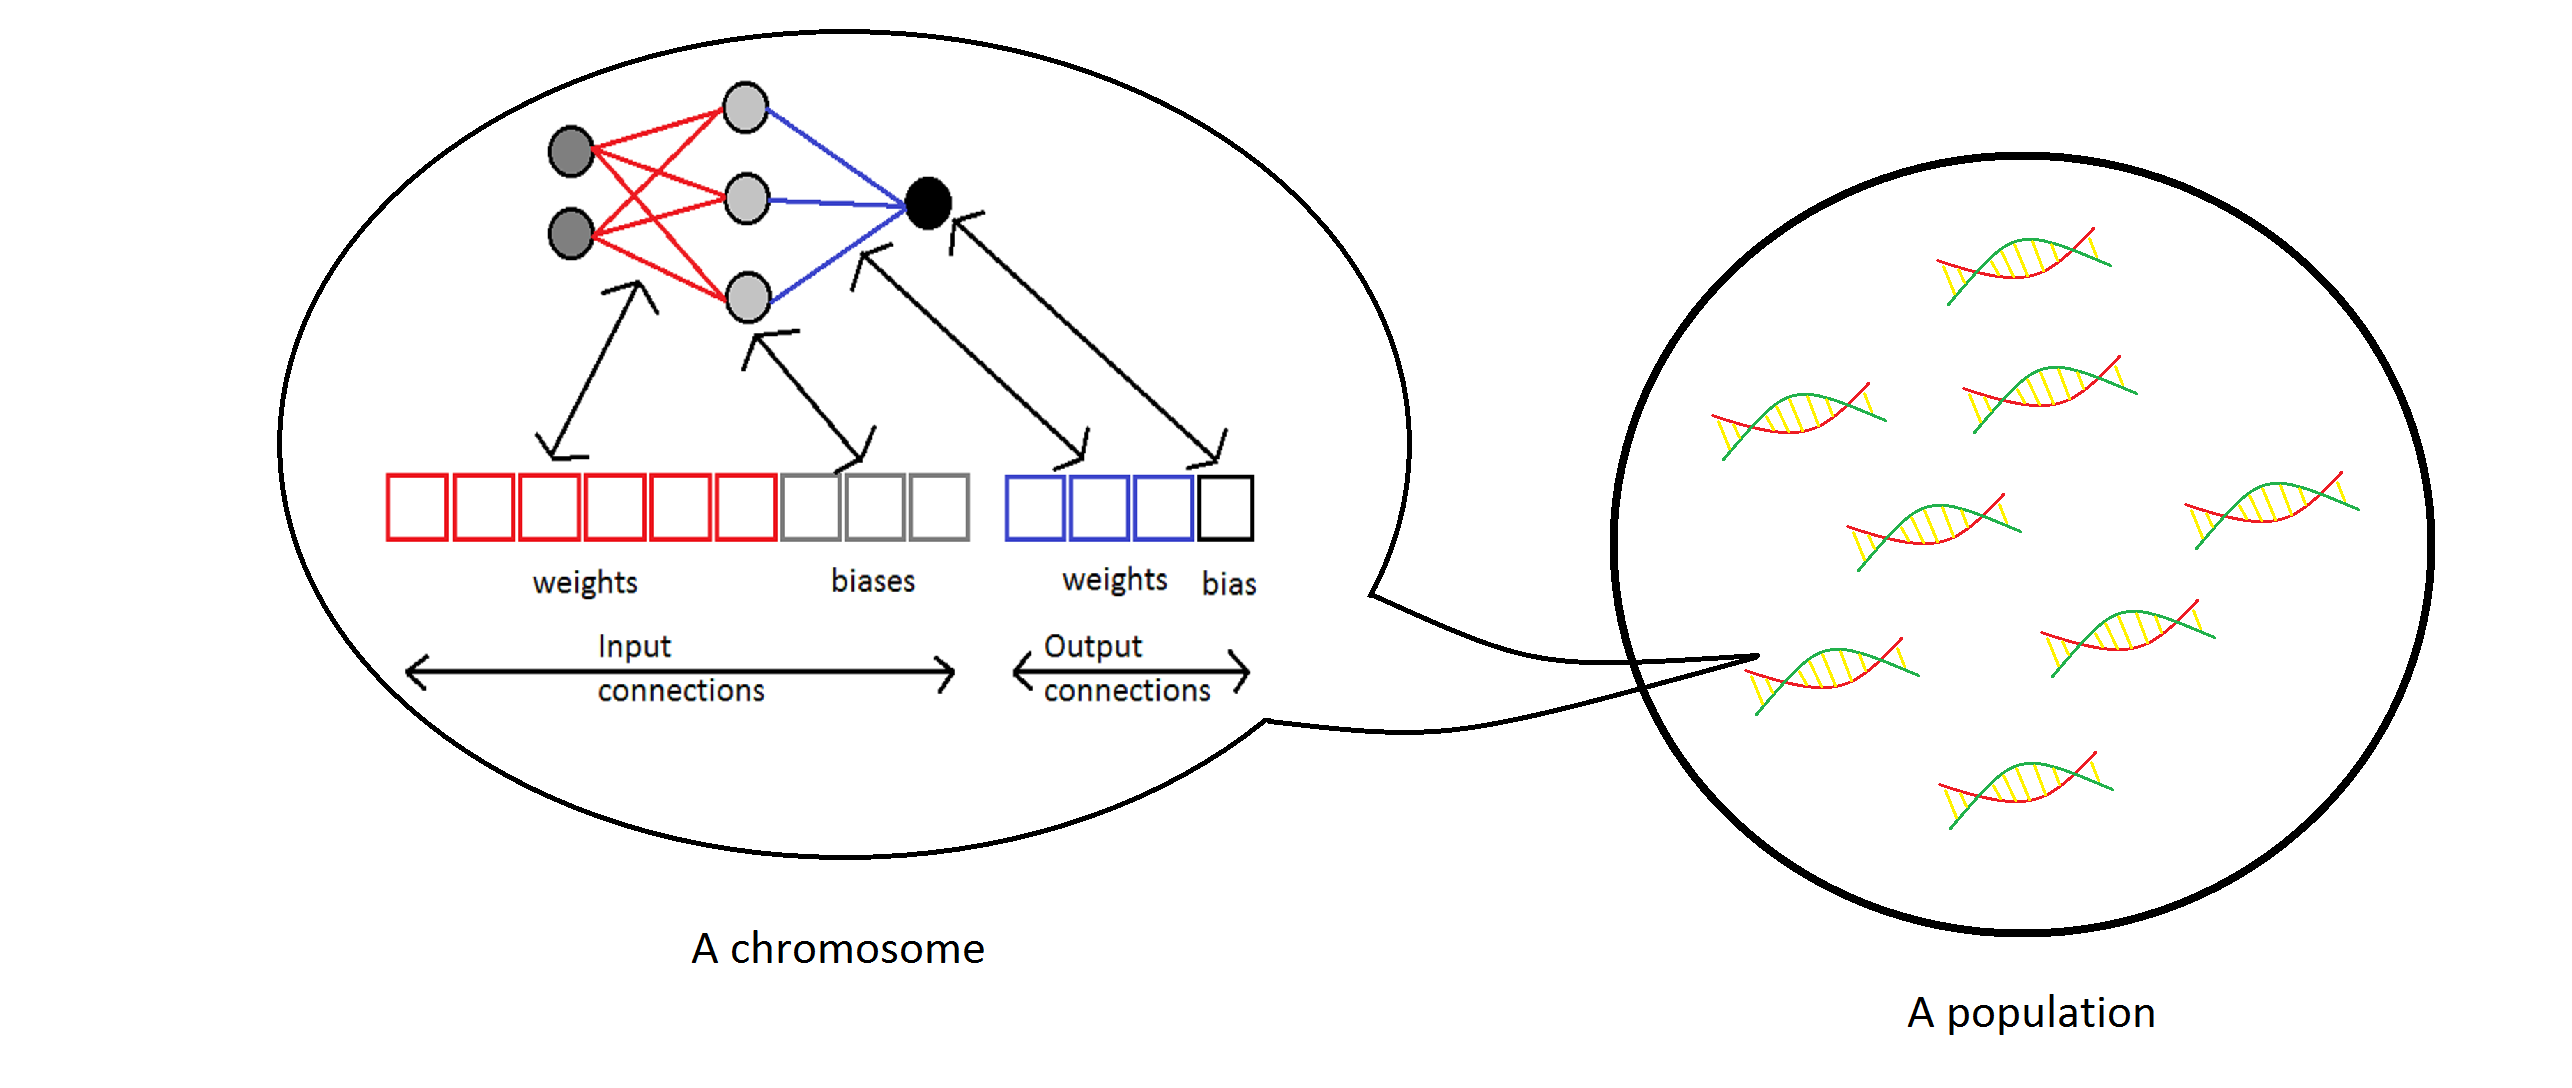
\includegraphics[width=\linewidth]{proposed_encoding.png}}}
    \caption{Quá trình mã hóa và giải mã policy tương wúng với các lớp của mạng}
    \label{fig:problem:policy-decode}
\end{figure}

Cách thức xây dựng không gian tìm kiếm chung như trong hình \ref{fig:problem:policy-decode} mặc dù đơn giản nhưng nó cũng đã chứng minh độ hiệu quả với hầu hết các thuật toán liên quan đến các ANN có cấu trúc giống nhau. Với phương pháp này, ANN sẽ được biểu diễn dưới dạng các lớp, tham số của các lớp sẽ lần lượt biểu diễn theo thứ tự trong nhiễm sắc thể. Phương pháp xây dựng cá thể cũng sẽ tương tự như bài toán huấn luyện nhiều ANN khác cấu trúc ở chương \ref{chap:problem}. Với bài toán này do sự khác nhau nằm ở bộ dữ liệu đầu vào (trạng thái của môi trường) nên cách thức xây dựng mô hình mã hóa, giải mã cũng sẽ đơn giản hơn. Có thể áp dụng phương pháp mã hóa trực tiếp. Mỗi cá thể sẽ có kích thước tương ứng với không gian tìm kiếm chung:
\begin{align}
    D_{chung} = \sum_{l={1,...L}}(h_{l-1}\cdot h_l + h_l)
    \label{rl:dmulti}
\end{align}
trong đó $h_1,h_2,...,h_k$ là kích thước của mỗi lớp ẩn, $l$ là số lượng lớp của mô hình mạng biểu diễn policy.

\subsection{Tiến hóa đa nhiệm đề xuất}

% \subsubsection{Tiến hóa đa nhiệm đề xuất}
% Với phân tích trong mục \ref{sec:multitask-rl}, trong RL ta chỉ cần chỉnh sửa tham số của môi trường một chút thì môi trường sẽ hoàn toàn thay đổi tương đương với một môi trường mới đối với \emph{agent}. Tuy nhiên ta lại không thể có một \emph{policy} thống nhất cho tất cả các môi trường trên. Để giải quyết vấn đề này, trước tiên tôi sẽ mô tả bài toán như sau:
% \begin{itemize}
%     \setlength\itemsep{0.01em}
%     \item Cho $K$ tác vụ $T_1, T_2, ..., T_K$.
%     \item Giả sử $h_k$ là bộ tham số môi trường tương ứng với tác vụ $T_k$, $h_j$ là bộ tham số môi trường tương ứng với tác vụ $T_j$ và $h_j \neq h_k$.
%     \item Mỗi tác vụ $k$ tương ứng với mô hình mạng Nơ-ron cùng cấu trúc khác bộ dữ liệu đầu vào là trạng thái của môi trường $h_k$
% \end{itemize}

% \emph{Nhiệm vụ đặt ra là tối ưu hóa đồng thời $K$ tác vụ này và tận dụng được độ tương đồng giữa chúng để tăng tốc độ tối ưu lẫn nhau}

% Như đã phân tích trong chương 2 MFEAII có hiệu quả cao trong việc khai thác những yếu tố ẩn có liên quan bên trong các tác vụ cũng như giảm sự trao đổi âm kém hiệu quả cho các tác vụ ít có sự liên quan. Tương ứng với mỗi môi trường, ta coi đó là một tác vụ. Bởi vậy nếu giải quyết các tác vụ đó đồng thời, MFEA-II có thể khai thác được sự tương đồng tiềm ẩn giữa các tác vụ và từ đó xây dựng được một \emph{policy} tối ưu, tổng quát cho mỗi tác vụ. Vì thế mỗi nhiễm sắc thể sẽ lưu trữ trong không gian tìm kiếm chung nên thông tin được biểu diễn bởi mỗi nhiễm sắc thể của các tác vụ khác nhau sẽ được MFEA-II tối ưu theo cách tương tự. Nói cách khác \emph{policy} của từng môi trường sẽ được học đồng thời bằng cách sử dụng MFEA-II. 

\subsubsection{Tính toán độ thích nghi đơn nhiệm}
\label{rl-fitness}


Các cá thể trong quần thể sẽ gắn với một tác vụ cần tối ưu hóa tương ứng với chỉ số kĩ năng của chúng. Với cá thể này ta sẽ phân tích ra bộ trong số $W$ và $b$ của mô hình mạng policy.
Từ $W$ và $b$ thu được tạo ra một mô hình policy, ta áp dụng policy này để tính tổng giá trị phần thưởng khi  đưa ra quyết định về các hành động tiếp theo tương tác với môi trường. Trong khuôn khổ của đồ án, tôi chỉ tập trung thực nghiệm trên các bài toán điều khiển đơn giản, do đó hàm đánh giá độ thích nghi được sử dụng sẽ là tổng phần thưởng khi áp dụng mô hình policy với bộ tham số hiện tại. Giá trị này càng lớn chứng tỏ độ thích nghi đơn nhiệm của cá thể $x$ càng cao, tức là nó sẽ có nhiều cơ hội được lựa chọn cho thế hệ tiếp theo hơn. Mô hình tính toán độ thích nghi đơn nhiệm của các cá thể thuộc từng tác vụ được biểu diễn như hình \ref{fig:problem:policy-ea}.

\begin{figure}[ht]
    \centering
    \scalebox{0.85}{\fbox{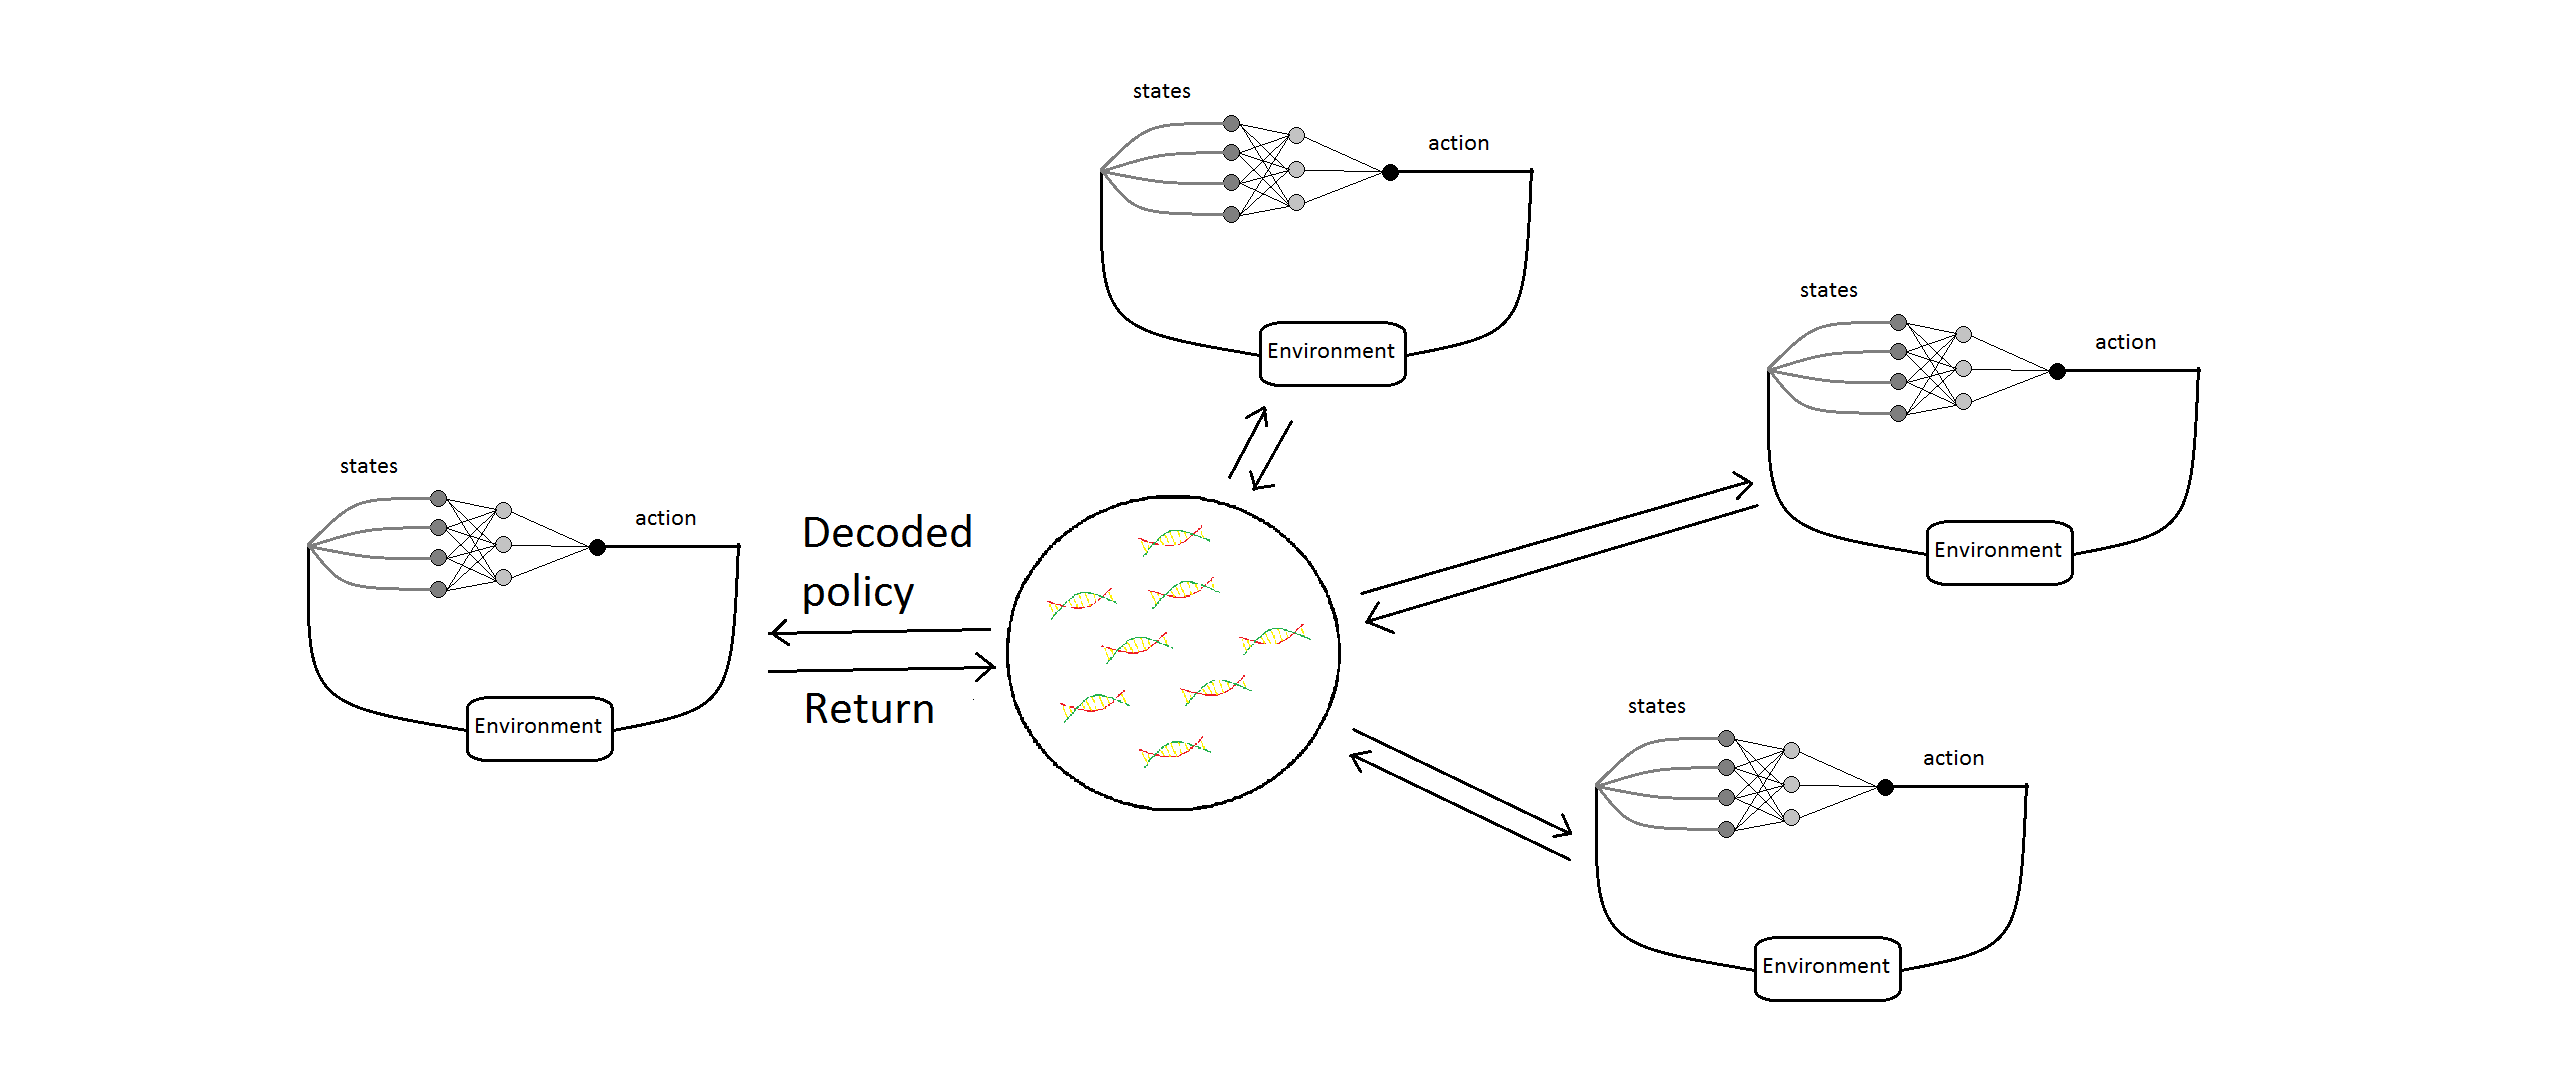
\includegraphics[width=\linewidth]{proposed_ea.png}}}
    \caption{Phương pháp tính toán độ thích nghi đơn nhiệm của từng tác vụ}
    \label{fig:problem:policy-ea}
\end{figure}

% Tuy nhiên cho đến hiện tại trong hiểu biết của tôi, MFEA-II là thuật toán mới nổi trội trong nhóm thuật toán tiến hóa nhưng chưa có nghiên cứu nào áp dụng MFEA-II để giải quyết vấn đề tương tự trong học tăng cường như tôi đã trình bày ở trên. Bởi vậy đồ án này là nỗ lực nghiên cứu của tôi để phát triển một hướng đi mới trong việc xây dựng lớp giải thuật tối ưu trong việc huấn luyện mô hình học tăng cường. Các kết quả thực nghiệm tôi sẽ trình bày chi tiết chương tiếp theo.

\subsubsection{Tiến hóa đa nhiệm đề xuất}
Về cơ bản giải thuật tiến hóa đa nhiệm đề xuất để huấn luyện nhiều mô hình học tăng cường đồng thời sẽ dựa theo khung thuật toán MFEA-II đã trình bày ở mục 1.4 và chiến lược tiến hóa đa nhiệm được mô tả trong giải thuật đề xuất huấn luyện nhiều ANN khác cấu trúc đồng thời tại chương \ref{chap:problem}.
Và cơ chế chọn lọc cá thể tối ưu trên không gian đa nhiệm theo đánh giá độ thích nghi vô hướng với những điều chỉnh phù hợp cho bài toán huấn luyện mô hình học tăng cường. Các bước giải quyết bài toán được biểu diễn theo thứ tự như trong giải thuật \ref{alg:proposed-alg2}
\begin{algorithm} [h!]
    \caption{Các bước chính của giải thuật tiến hóa đa nhiệm huấn luyện nhiều mạng neural khác cấu trúc}
    \begin{algorithmic}[1]
        \State Xác định không gian biểu diễn chung theo giải thuật \ref{rl:dmulti}
        \State Khởi tạo các cá thể ngẫu nhiên của từng tác vụ theo phân phối chuẩn \ref{h-multi}
        \State Gán chỉ số kỹ năng cho mỗi cá thể
        \State Đánh giá giá trị thích nghi đơn nhiệm mỗi cá thể theo chỉ số kỹ năng tương ứng bằng cách tính tổng reward thu được từ các mô hình policy xây dựng từ cá thể
        \For{Điều kiện dừng}
            \State Xáo trộn thứ tự ngẫu nhiên các cá thể trong quần thể $P$
            \State Xác định tập các cá thể thuộc từng tác vụ
            \State Học ma trận xác suất ghép cặp $RMP$ giữa các cặp tác vụ với tập các cá thể hiện tại
            \For{Duyệt hết các cá thể trong quần thể}
                \State Chọn ngẫu nhiên $p_1, p_2$ trong quần thể $P$
                \State Lai ghép, đột biến bằng cách tổ hợp $p_1, p_2$
                \State Đánh giá giá trị thích nghi đơn nhiệm cho mỗi cá thể mới bằng cách tính tổng reward thu được từ các mô hình policy xây dựng từ cá thể
                \State Tính toán độ thích nghi vô hướng của mỗi cá thể
                \State Chọn lọc cá thể
            \EndFor
        \EndFor
    \end{algorithmic}
    \label{alg:proposed-alg2}
\end{algorithm}

\subsubsection{Phép lai ghép đột biến trong không gian chung}
Giống như bài toán huấn luyện nhiều ANN đồng thời trong chương \ref{chap:problem} sử dụng phép lai ghép SBX và phép đột biến PMU để làm phép tìm kiếm cơ sở và không sử dụng bất cứ phép biến đổi nào dựa trên đạo hàm. Cũng theo lẽ đó, tiến hóa đa nhiệm đề xuất trong đồ án với bài toán này cũng không sử dụng bất cứ phép biến đổi nào dựa trên đạo hàm. Cụ thể các phép lai ghép, đột biến được sử dụng là SBX và PMU. Và để đảm bảo nguyên tắc các cá thể con cái sinh ra là parent-centric, chỉ số phân phối SBX và tỉ lệ đột biến PMU đều cần có giá trị đủ lớn.

\subsubsection{Học ma trận $RMP$ trên số chiều của không gian tìm kiếm chung}
Với bài toán này do tác vụ có số chiều giống nhau nên việc học ma trận xác suất lai ghép ngẫu nhiên $RMP$ cũng sẽ giống với giải thuật \ref{alg:rmp} được đề cập trong chương \ref{chap:problem}. Hay nói cách khác ma trận $RMP$ sẽ được học dựa trên số chiều của không gian tìm kiếm chung.
\\[1cm]
Đồ án này là nỗ lực nghiên cứu phát triển một hướng đi mới trong việc xây dựng lớp giải thuật tối ưu trong việc huấn luyện nhiều ANN và cụ thể với bài toán huấn luyện nhiều mô hình học tăng cường đồng thời. Qua đó mong muốn chứng minh rằng các phương pháp tiến hóa đặc biệt là MFEA-II là hiệu quả trong việc giải quyết những bài toán kể trên. 
Các kết quả thực nghiệm tôi sẽ trình bày chi tiết chương tiếp theo sẽ phần nào chứng minh được mục tiêu mà đồ án đề ra.
